\documentclass[sectioncirclenumberstyle]{le2iutbmbeamer}
\usepackage{siunitx}
\usepackage{algpseudocode}
\usepackage{multicol,multirow,colortbl,smartdiagram,bm}
\usepackage{tabularx}
\usepackage{booktabs}
\usepackage{ctex}
\hypersetup{
	pdfauthor = {汪卫},
	pdfsubject = {MIK\TeX{}安装与更新配置},
	pdfkeywords = {\LaTeX,安装配置},
	pdfpagemode=FullScreen,
	pdfcreator = {}
}
\usefonttheme{professionalfonts}
\title{MIK\TeX{}安装与更新配置}
\subtitle{ 北理工硕博论文模板编译环境配置}
\author[汪卫]{汪卫}
\authordescription{wweibit@163.com}
\institute[BIT]{北京理工大学宇航学院}
\instituteurl{https://github.com/qiuzhu}


\subject{模板编译环境简介}

\finalslidetext{欢迎同学建议!}

\usefootlinewithsections
\useheaderlinewithuserlogo{bit.pdf}
\pgfdeclareimage[height=.2cm]{fakele2ilogoinpartners}{le2ilogo}
\pgfdeclareimage[height=.2cm]{fakeutbmlogoinpartners}{utbmlogo}
\pgfdeclareimage[height=.2cm]{fakeubfclogoinpartners}{ubfclogo}
\pgfdeclareimage[height=.2cm]{fakecnrslogoinpartners}{cnrslogo}
\pgfdeclareimage[height=.25cm]{fakele2ilogointitle}{le2ilogoinv}
\pgfdeclareimage[height=.25cm]{fakemaglogointitle}{multiagentlogoinv}
\pgfdeclareimage[height=.25cm]{fakeutbmlogointitle}{utbmlogoinv}
\pgfdeclareimage[height=.25cm]{fakeubfclogointitle}{ubfclogoinv}
\pgfdeclareimage[height=.25cm]{fakecnrslogointitle}{cnrslogoinv}
\pgfdeclareimage[height=.25cm]{fakeuserlogointitle}{utbmlogo}

\makeatletter
\let\fakebackground\beamer@theme@leiiutbm@outer@background
\makeatother

\makeatletter
\let\fakeoldunderline\beamer@theme@leiiutbm@oldunderline
\makeatother

\newcommand{\fakeslide}[3][fakele2ilogointitle]{
	\framebox{\begin{minipage}{.4\paperwidth}
		\begin{picture}(0,90)
			\put(-3,81.25){\scalebox{0.41}{\fakebackground}}
			\put(10,86){\textcolor{white}{\tiny #2}}
			\ifthenelse{\equal{a#1}{a}}{}{\put(-1,84.5){\pgfuseimage{#1}}}
			#3				
			\put(100,-1){
				\pgfuseimage{fakele2ilogoinpartners}\hspace{0.05cm}\pgfuseimage{fakeutbmlogoinpartners}\hspace{0.05cm}\pgfuseimage{fakeubfclogoinpartners}\hspace{0.05cm}\pgfuseimage{fakecnrslogoinpartners}}
		\end{picture}
	\end{minipage}}
}

\begin{document}

%%%%%%%%%%%%%%%%%%%%%%%%%%%%%%%%%%%%%%%%%%%%%%%%%
\begin{frame}{模板编译环境简介}
目前latex的编译发行版比较多,常用的有Texlive 和 Mik\TeX{}套装,但Texlive 套装(截至目前版本2017)实在超大,很多宏包对于只写毕设的人来说也用不到,Texlive比较好安装,这里不再演示,下面关于Mik\TeX{} 介绍:
\begin{itemize}
    \item  Mik\TeX{}基础包只有200M不到;
    \item  可以在线安装缺失宏包;
    \item 目前只在Windows下版本文档;
    \item 更新机制对大陆不友好,经常宕机,需要手动切换
\end{itemize}
\alert{对于想减少安装体积,体验Mik\TeX{}可以往下看,否则会绕过}
\begin{alertblock}{中文输出方案}
对于中文解决方案,目前采用XeCJK或者ctex宏包,过去的Ctex套装已经过时,本硕博模板不会通过
\end{alertblock}
\end{frame}


%%%%%%%%%%%%%%%%%%%%%%%%%%%%%%%%%%%%%%%%%%%%%%%%%
\tableofcontentslide

%%%%%%%%%%%%%%%%%%%%%%%%%%%%%%%%%%%%%%%%%%%%%%%%%
\section{Mik\TeX{}安装步骤}
\subsection{下载与安装}
\begin{frame}{Mik\TeX{}下载地址}
		推荐清华大学镜像站下载,支持ipv6,可以免流量下载,截止目前,版本号是6361
       下载地址如下:\alert{此处给出的是64位的,32位的自行去下载}
   
    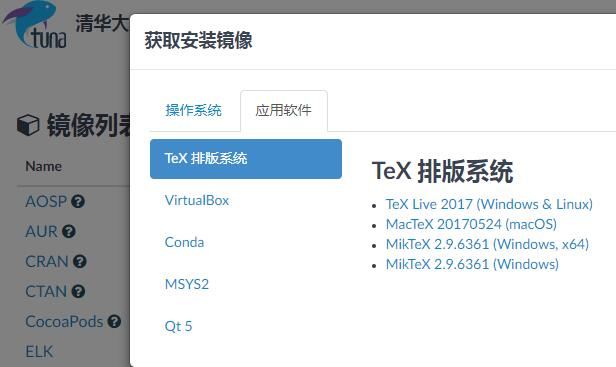
\includegraphics[width=0.7\linewidth]{figures/11}
    
       \url{https://mirrors6.tuna.tsinghua.edu.cn/CTAN/systems/win32/miktex/setup/basic-miktex-2.9.6361-x64.exe}{Mik\TeX}
       
\end{frame}

\subsection{安装方法}

\begin{frame}{安装方法}
安装exe文件,一路点击确认即可,自己可自定义安装盘
\centering
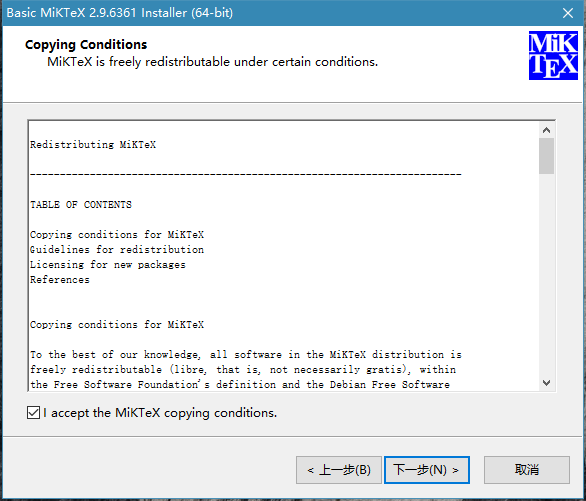
\includegraphics[height=0.6\linewidth]{figures/1}
\end{frame}

\section{Mik\TeX{}配置}
\begin{frame}{安装配置}
安装完成后,\alert{一定需要配置才能使用,因为6361版本出现了和fontspec宏包冲突的bug}:
首先需切换到大陆源,或者就近的源,一般选择清华大学源:
\centering
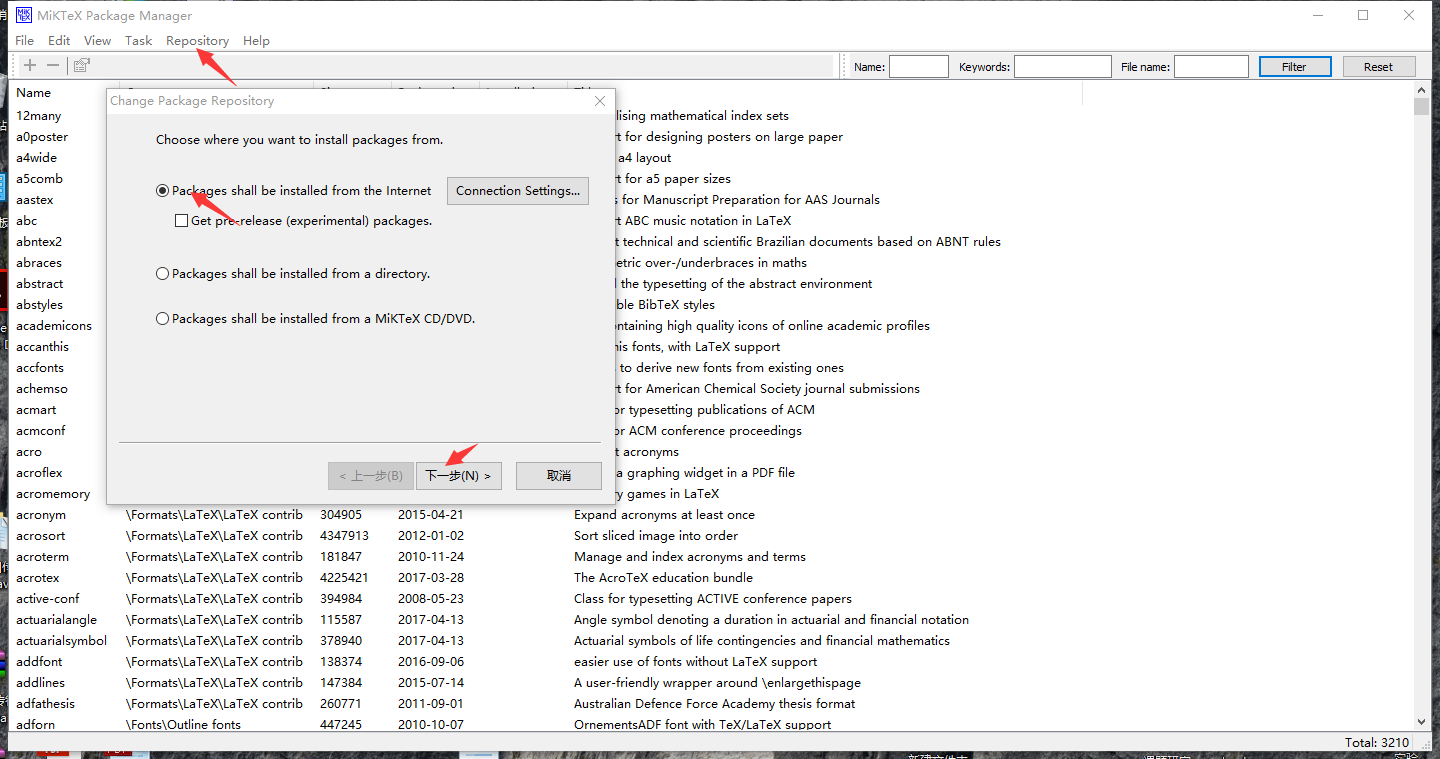
\includegraphics[height=0.6\linewidth]{figures/3}
\end{frame}

\begin{frame}{安装配置注意事项}
\begin{alertblock}{更新源注意事项}
    这也就是Mik\TeX{}最无语的地方,对大陆不友好,经常清华大学的源连接不上,这时候切换到另外一个就近的源即可
    
\end{alertblock}
\centering
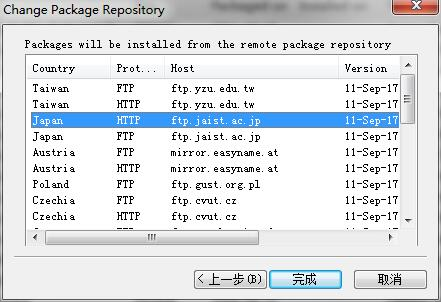
\includegraphics[height=0.5\linewidth]{figures/12}
\end{frame}
\begin{frame}{Mik\TeX{}主程序更新配置方法}

\alert{6361版本存在bug,需要更新主程序,建议一周习惯性更新一次}:

菜单 --》 Miktex  update
\centering
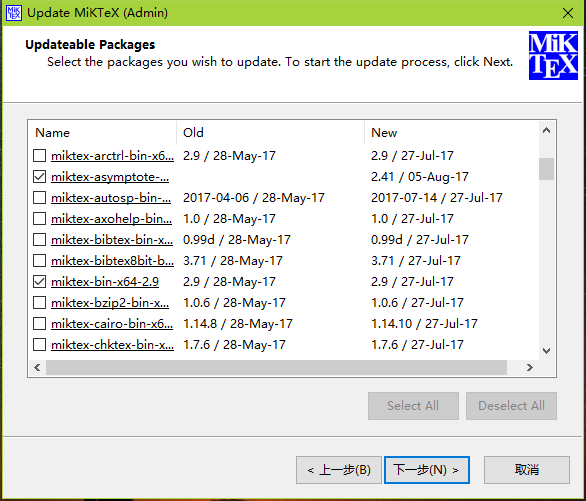
\includegraphics[height=0.6\linewidth]{figures/7}
\end{frame}

\section{硕博模板的编译}

\begin{frame}{模板的下载}

首先在GitHub下载最新的模板,可以在主页\url{https://github.com/BIT-thesis/LaTeX-template}打包下载,或者利用git 工具 ,git clone 下来:

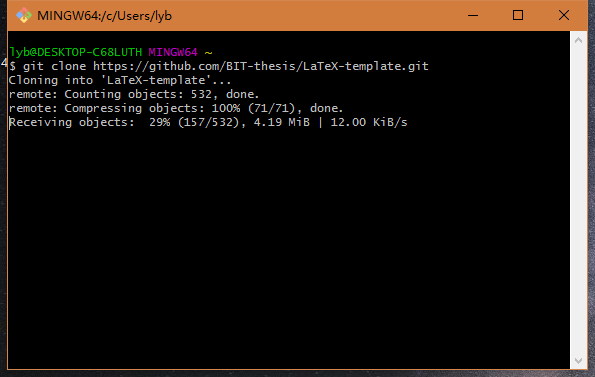
\includegraphics[width=0.7\linewidth]{figures/4}
\end{frame}

\begin{frame}{模板的下载}
本模板采用Xelatex编译,利用编辑器编译时候需要改变默认引擎,推荐采用texstudio,智能编译器,无需记忆命令,不过下面图方便就以默认的texwork作为演示:
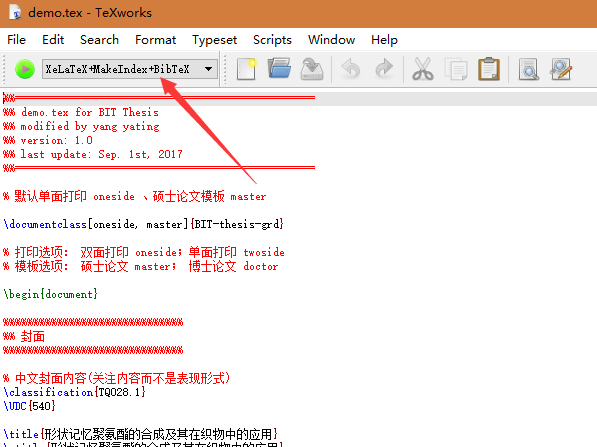
\includegraphics[width=0.7\linewidth]{figures/5}
\end{frame}

\begin{frame}{缺少宏包的自动下载安装}
缺少宏包的自动下载安装也是Mik\TeX{}最强大之处,本模板设计多个宏包,所以第一次编译安装在线宏包需要一段时间,耐心等待,一次不成功,多搞几次:

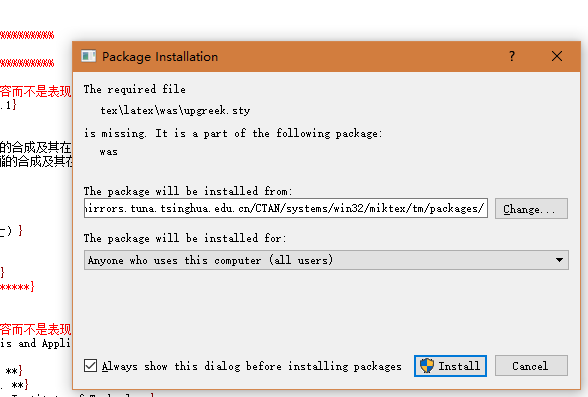
\includegraphics[width=0.7\linewidth]{figures/6}

\alert{弹窗一定要点确认!!!!!}
\end{frame}
\end{document}
